\label{chap:analisi}
\section{Analisi esplorativa}

% serie storiche

\begin{definition}
    Una serie di dati è una sequenza ordinata di punti dati, ed esprime la
    dinamica di un certo fenomeno nel tempo. Quando questi dati sono ordinati
    in base al tempo, si parla di una \textbf{serie storica} (o
    \textbf{temporale}).
    Indipendentemente dal criterio utilizzato per ordinarli, i punti dati sono
    registrati seguendo intervalli di tempo equispaziati. Le serie temporali
    possono essere di due tipi: \textbf{univariate}, che coinvolgono una
    singola variabile misurata nel tempo, e \textbf{multivariate}, dove più
    variabili sono misurate contemporaneamente.
\end{definition}

Nel caso dei dati di monitoraggio dei job in esecuzione nella tabella
\texttt{hj}, ogni riga della tabella può essere visto come un punto in una
serie storica multivariata. Poiché in \texttt{hj} abbiamo più job che sono
stati messi in esecuzione da HTCondor allora abbiamo più serie multivariate
che condividono le stesse variabili.

\begin{figure}[ht]
    \centering
    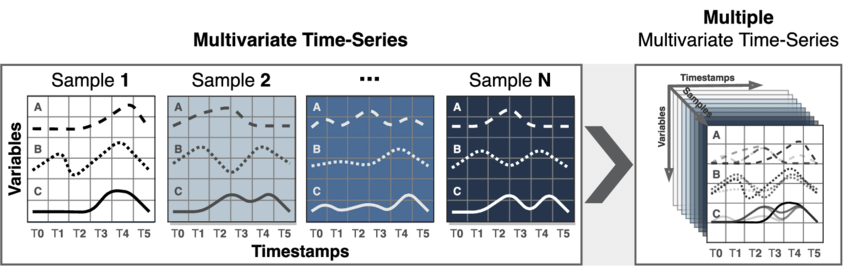
\includegraphics[width=0.9\linewidth]{A-multiple-multivariate-time-series}
    \caption[legenda elenco figure]{A multiple seri}\label{fig:prima}
\end{figure}

% funzioni monotone crescente

% frequenza di campionamento ogni 3 minuti ma ogni 15 minuti viene aggiornato

% i gruppi hanno distribuzioni diverse

% job di durata molto variabile

% numero di jobs e runtime all'ora

% Analizzando le prime 48 ore e raggruppando tutti i jobs successivi alla
% 48-esima ora, si nota che:
% i jobs più brevi di un'ora sono una gran quantità e hanno un altissimo tasso
% di fallimento, ma il loro tempo speso sulle macchine è minore dell'1% del
% totale speso dai jobs di durata maggiore. nella prima ora la maggior parte dei
% jobs dura meno di 5 minuti e probabilmente sono "tentativi", ovvero jobs che
% non hanno le condizioni necessarie per poter partire non verranno considerati
% i jobs con runtime < 1h, poichè non rilevanti per il sistema.

\section{Job Zombie Prediction}

% tempo di timeout code LHC e code non LHC

% le code LHC sono quelle caratterizzate maggiormente da job zombie 

% tempo perso per job zombie 

% sono separabili questi job dai job normali e su che base

\section{Preparazione dei dati per il task di ML}
\subsection{Trasformazione delle serie storiche multivariate multiple}

% padding e truncate delle serie storiche 

% avg pooling

% tabular transformation

% tensor transformation

\subsection{Creazione delle feature}

% job work type

% job type

% one hot encoding

\subsection{Labeling dei dati}
\subsection{Tecniche di bilanciamento dei dati}

% undersample

% oversample

% class weighting in loss function

% metriche
